\documentclass[hyperref={pdfencoding=unicode, unicode=true}, xcolor=dvipsnames]{beamer}
%\usecolortheme[named=Maroon]{structure}
\usetheme{Berlin}

\usepackage[utf8x, utf8]{inputenc}
\usepackage{ucs}
\usepackage[english]{babel}
\usepackage{graphics}
\usepackage{booktabs}

\hypersetup{
	pdftitle={Resource-light Acquisition of Inflectional Paradigms},
	pdfauthor={Radoslav Klíč},
	pdfsubject={Resource-light Acquisition of Inflectional Paradigms}
}

\newcommand{\eg}{e.g.,~}

\title[Resource-light Acquisition of Inflectional Paradigms]{Resource-light Acquisition of Inflectional Paradigms}
\author{Radoslav Klíč and Jirka Hana}
\institute{Geneea Analytics / MFF UK Praha}
\date{}

\begin{document}

%\AtBeginSection[]
%{
%  \begin{frame}<beamer>
%    \frametitle{Outline}
%    \tableofcontents[currentsection,currentsubsection]
%  \end{frame}
%}

\begin{frame}
\titlepage
\end{frame}

\begin{frame}{Outline}
	\tableofcontents
\end{frame}

\section{Introduction}

\begin{frame}{Introduction}

\begin{itemize}

\item Morphology analysis necessary (IR etc.) but manual approach is expensive.

\item We assume limited resources: plain text corpus and consultation with a native speaker.

\item Our approach: modification and extension of Paramor, an unsupervised paradigm learner.

\item We try to `nudge' it towards correct analysis
\end{itemize}

\end{frame}

\begin{frame}{Paradigms}

\begin{itemize}
\item Classical Czech paradigms have slots for all combinations of relevant morphological categories.

\begin{scriptsize}
\begin{center}
\begin{tabular}{lll}
\toprule \bf Case & \bf Singular & \bf Plural \\ \midrule
nom & mat\textbf{k}+a & mat\textbf{k}+y \\
gen & mat\textbf{k}+y & mat\textbf{ek}+0 \\
dat & mat\textbf{c}+e & mat\textbf{k}+ám\\
acc & mat\textbf{k}+u & mat\textbf{k}+y \\
voc & mat\textbf{k}+o & mat\textbf{k}+y \\
loc & mat\textbf{c}+e & mat\textbf{k}+ách \\
inst & mat\textbf{k}+ou & mat\textbf{k}+ami \\
\bottomrule
\end{tabular}
\end{center}
\end{scriptsize}

\item Low knowledge of grammar of the given language $\rightarrow$ simplified paradigms defined as a set of suffixes + set of stems e.g., (\emph{a, y, e, u, o, ou, 0, ám, ách, ami}) + (\emph{žen, matk, \ldots})

\end{itemize}
\end{frame}

%\begin{frame}{}

%Work done in the thesis:
%\begin{itemize}
%\item Modification of Paramor, an unsupervised morphology learner by Monson (2009),  to: \begin{itemize}
%    \item accept manually provided inflections with marked morpheme boundary.
%    \item handle allomorphy.
%\end{itemize}
%\item A framework for hierarchical clustering using modified edit distance and other string distance metrics.
%\end{itemize}
%
%\end{frame}

\section{Paramor}

\begin{frame}{Paramor -- Schemes}
\begin{itemize}
\item All splits of all words in the corpus $\rightarrow$ \emph{c-stems} and \emph{c-suffixes}
\item In Paramor, partial paradigms are modelled by \emph{schemes}.
\item Scheme defined by a set of c-suffixes \eg (\emph{0, ed, ing, s}).
\item scheme's stem set $\rightarrow$ all c-stems which form a word in the corpus with all the scheme's suffixes.
\item Observation: adding a suffix cannot increase the number of scheme's adherent stems.
\end{itemize}
\end{frame}

\begin{frame}{Scheme lattice}
\vspace{-8pt}
\begin{center}
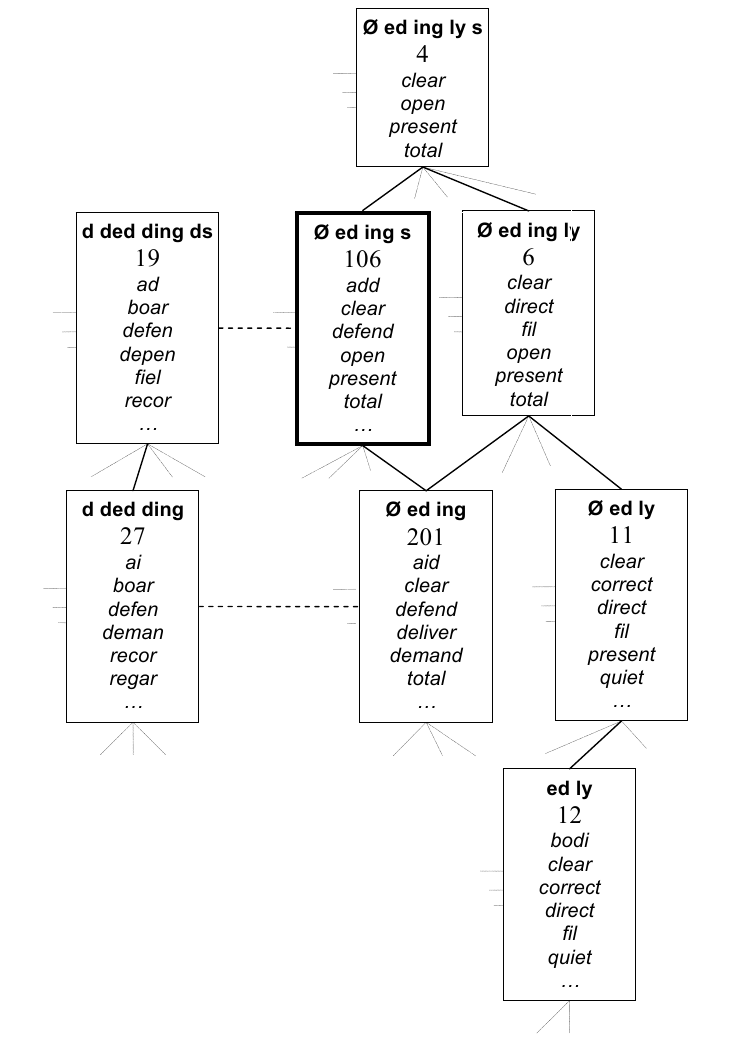
\includegraphics[scale=0.25]{schemeLattice.png}
\end{center}

\end{frame}


\begin{frame}{Paramor algorithm}
\begin{itemize}
\item Bottom-up search. Starts with single-suffix schemes and ascends the lattice. Stops when the c-stem ratio drops below 0.25.
\item Scheme clustering. Join similar schemes into scheme clusters. Similarity $\rightarrow$ similarity of (stem, suffix) pair sets. For example, schemes (\emph{0, ly, ness}) and (\emph{0, ly, er, est}) could be merged, as they share a lot of stem-suffix pairs like \emph{deep + 0}, \emph{deep + ly}.
\item Scheme cluster pruning.
\end{itemize}
\end{frame}

\section{Seeding}

\begin{frame}{Seeding}
\begin{itemize}
\item Modified Paramor accepts manually entered input in the form of inflected word forms with marked morpheme boundary.
\item Seed example: \emph{matk/matc/matek} + \emph{a, u, y / e / 0}
\item Usage: \begin{itemize}
    \item Add two-suffix schemes to the initial scheme set for bottom-up search.
    \item Protect some scheme clusters from discarding.
    \item Induction of allomorphy rules.
\end{itemize}
\end{itemize}
\end{frame}

\section{Allomorphy}

\begin{frame}{Allomorphy}
\begin{itemize}
\item Allomorphy -- more surface variants of a stem.
\item Problem: try adding \emph{-e} suffix to a scheme \emph{(matk, noh)} + \emph{(a, y, u, ou)}
\item Oh no! neither \emph{matke} nor \emph{nohe} is in the corpus. (Although \emph{matce} and \emph{noze} are)
\item Leads to \begin{itemize}
    \item Incomplete schemes
    \item Schemes with shifted morpheme boundary. \emph{(mat)} + \emph{(ka, ky, ce)}
\end{itemize}
%\item Paramor does not recognise allomorphic stems. As a result, suffixes triggering phonological changes are often not selected in the bottom-up search, because they form words with different surface stems. 
%\item For example, let's assume the bottom-up search on a Czech corpus reached a scheme \emph{(a, y, u, ou)} with stems like \emph{matk, noh} and tries to add \emph{-e} suffix.
%\item In this case, stems where a phonological change is triggered (like \emph{matk} $ \rightarrow $ \emph{matc}, \emph{noh} $ \rightarrow $ \emph{noz}) will drop out after adding \emph{-e}, which significantly decreases the c-stem ratio and causes the search to stop before adding \emph{-e}.
\end{itemize}

\end{frame}

\begin{frame}{Allomorphy -- usage of the seed}
\begin{itemize}
\item Induction of stem equivalence rules.
\item From a seed entry 
\begin{quote}
\emph{politik/politic + a, u, ovi, em, y, ů, ům / i, ích}
\end{quote}
we generate:
\begin{quote}
$*k \leftrightarrow *c$ / \{\emph{a, u, ovi, em, y, ů, ům}\}, \{\emph{i, ích}\}
\end{quote}
\end{itemize}

\end{frame}

%\section{Edit distance}
%
%\begin{frame}{Edit distance}
%In my clustering framework, I have experimented with modified Levenshtein distance, for which:
%\begin{itemize}
%\item the cost of operations linearly decreases with the position in the string where it occurs. (cost of \emph{walk} $\rightarrow$ \emph{talk} higher than \emph{talked} $\rightarrow$ \emph{talker})
%\item the costs for diacritics adding/removing and vowel changes are lower than for other operations. (\emph{hranici} $\rightarrow$ \emph{hranicí}, \emph{žena} $\rightarrow$ \emph{ženy})
%\end{itemize}
%\end{frame}

\section{Results}

\begin{frame}{Evaluation}
\begin{itemize}
\item Most common `gold' data: lemmatised corpora
\item For each word pair ($w_1$, $w_2$)
    \begin{itemize}
    \item Do $w_1$ and $w_2$ belong to the same lemma?
    \item Is there a scheme cluster generating both $w_1$ and $w_2$?
    \end{itemize}
\item Count true/false positives/negatives $\rightarrow$ precision and recall $\rightarrow$ F-score.
\end{itemize}
\end{frame}

\begin{frame}{Results}
F-score obtained with and without seeding:

\begin{center}
\begin{tabular}{lrr}
\toprule
\bf Corpus & \bf no seed & \bf seed \\
\midrule
cz  & 69.63 & \bf 72.99 \\
si  & 74.83 & \bf 75.61 \\
de  & 63.98 & \bf 64.52 \\
cat & 62.74 & \bf 65.95 \\
\bottomrule
\end{tabular}
\end{center}
\end{frame}

\begin{frame}{Some problems}
\begin{itemize}
\item Derivation vs inflection (\emph{výuk + a}, \emph{výuk + ový})
\item Prefixes (\emph{ne-}, \emph{nej-})
\end{itemize}
\end{frame}

%\begin{frame}{Discussion}
%
%Problems with German:

%\begin{itemize}
%\item Stem-internal changes (\emph{Mutter}/\emph{M\"{u}tter})
%
%\item Compounds -- creation of schemes as (\emph{0, organisation}) or (\emph{0, gruppe})
%\end{itemize}
%\end{frame}
%
%\begin{frame}{Future work}
%\begin{itemize}
%
%\item Rules for stem-internal vowel change (\emph{Mutter}/\emph{M\"{u}tter})
%
%\item More information sources (context, semantics, \ldots)
%
%\end{itemize}
%\end{frame}


\end{document}